\documentclass[../main/main.tex]{subfiles}

\newdate{date}{25}{03}{2020}



\begin{document}

\section{Lecture 5}
 \displaydate{date}. Compiled:  \today. Alice.
 

\subsubsection{Slide 82}

\begin{figure}[h!]
\centering
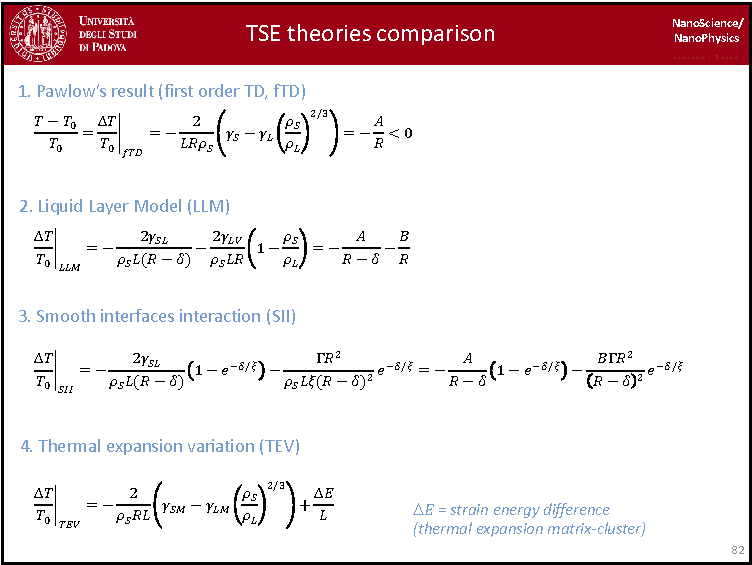
\includegraphics[page=1,width=0.9\textwidth]{../lessons/pdf_file/5_lesson.pdf}
\end{figure}


In this slide we write a briefly recap of what we have seen in the previous lectures.

In particular, for \textbf{thermal expansion variation} (TEV): if we have a nanoparticle which is not embedded in vacuum or which is in equilibrium with its vapour, the solid matrix can produce additional effects on melting temperature. I f there is a mechanical coupling between matrix and nanoparticle we can have along the first order therm, another additional term  \( \frac{\Delta E}{L} \) which is an offset triggered by \( \Delta E \) ad can be due to the difference thermal expansion matrix-cluster or hydrostatic pressure of matrix onto nanoparticle.


\newpage

\subsubsection{Slide 83}

\begin{figure}[h!]
\centering
\includegraphics[page=2,width=0.9\textwidth]{../lessons/pdf_file/5_lesson.pdf}
\end{figure}

Implantation means that we produce ions and we want to insert them into the matrix (in this case is a silica matrix). They can be accellerated trough a differential potential (320keV in this case). The fluence is the number of ions reaching the unit of surface.
Implantation is a stocastic process in which the interaction ion-matrix produce binary collision. Hence we have defect and feflaction of trajectory (we have a random path with momentum in direction perpendicular to the surface).

Let us consider the four pictures that describes the evolution of melting temperature in Indium where the scale we are considering is of \( 50 \)nm for all the figures.

\begin{itemize}
\item 298 K. This is the picture at room temperature. This image corresponds to the cross section of Indium nanoparticle in silica. Above we have the surface and ions are incoming perpendicularly to it. In particular, the ion stops in average at the same points and the average pf all those points for all the atoms is called the \textbf{projected range} while the dispersion around this value is called \textbf{straggling}. This will produce a gaussian-like profile in the concentration of ions in substrate. This is able to promote nucleation and growth. Indeed if we have a sufficiently high concentration of an element in another matrix we can produce precipatated nanoparticles.

In this figure we see the metallic indium nanoparticle, which has a tetragonal cell and we note that the shape is elongated in the direction of the momentum.

\item 443 K. The temperature now is above the melting temperature of the bulk, however we still see nanoparticles.

\item 888 K. It is twice the bulk melting temperature. We start to see ghost particles. When we look at cross section sample of our implanted silica we thin the sample down to electron transparency. The tickness in the perpendicular direction (with respect to the image) is 100nm at most.
For that reason we do this kind of observation: the metallic cluster above the surface find a path for high diffusing and toward the new face produce by the thinning of the sample.

\item 983 K. We see that most cluster disappear.

\end{itemize}

\newpage

\subsubsection{Slide 84}

\begin{figure}[h!]
\centering
\includegraphics[page=3,width=0.9\textwidth]{../lessons/pdf_file/5_lesson.pdf}
\end{figure}


We want to analyze the topological properties of nanoparticles. We see histograms of the larger radius of the larger axis of the nanoparticle for different temperatures.
Increasing temperature the distribution becomes more homogeneous and we can see the two main components (gaussians).
Basically the largest component is more or less constant, while the smaller component moved toward larger one. We see a very interesting result and we will see how to interpret this result when we do a coarse grain of the system.
When we are experimenting increasing the temperature we have thermodynamic competition of nanoparticles with different size. The larger is the size the better is the theromdynamic stability.
The smaller nanoparticles tends to increase their size and to stabilize even further the already stabòe nanoparticles present in the system in that specific moment. We will see how to describe it.

Hence, in conclusion the stabilization of largest nanoparticles means theromdynamic stability.

\newpage

\subsubsection{Slide 85}

\begin{figure}[h!]
\centering
\includegraphics[page=4,width=0.9\textwidth]{../lessons/pdf_file/5_lesson.pdf}
\end{figure}

In these figures we can see diffraction of electrons: in particular the cross section in the reciprocal space. Each point is the result of a set of planes producing electron diffraction toward that direction in the reciprocal space.
We can also see a metallic block that cause the stop of electrons which did not suffered from electron diffration (so they go on a straight line without changing direction).

We see ring-like structures because of random orientation of particles. Instead of having a single reciprocal space we see circles of points which are all having the same distance with respect to the center. We can label rings according to the miller index (index as tetragonal centered clusters are consistant with bulk structure of indium).

When you have a discontinuous rings is because when you do electron diffraction you sample a non infinite set of nanoparticles.

Increasing the temperature (150°) we have a more distributed intensity of the pattern because we have much larger vibrational energy. Atoms vibrate a lot around their equilibrium position (we have a thermal broadening of the rings due to the temperature, \textbf{bywaller factor}).

If we go above the bulk melting temperature (170°) we still see some spots, but the number is decreased. However you still see nanoparticles.
If indium becomes liquid you should see some high diffusion of particles with respect their original site. Instead there is this kind of effect of blistering. Particles are trapped in the blister created by the matrix which is able to confine the liquid atoms in their position.

Going higher in temperature all the spots disappear and we have a complete melting of the particle.
Important: it is reached above the bulk melting temperature!
In contrary with what we expect by a purely thermodynamic size effect. But this can be understood exactly in the effect of the matrix compression onto the nanoparticle.
The matrix is able to retard the complete melting up to a temperature larger than the melting one (we will describe it quantitively with thermal expansion variation) with respect to the two system: silican matrix and indium metallic cluster.

Try to see what is going on decreasing the temperature. We see that the process is not completely reversable. Indeed for 45° we see only some spots. The vast majority of nanoparticles still remaing in this phase even at this temperature.

To recover the original pattern we have to go very very down in temperature and we still not reach completely the original structure.
This is a kind of \textbf{isteresis loop} that we obtain on going from \( 27° \rightarrow 150° \rightarrow 174° \rightarrow 45° \rightarrow 25°\).  So we have to go again to the room temperature to see again a significant number of cristallying.

\newpage

\subsubsection{Slide 86}

\begin{figure}[h!]
\centering
\includegraphics[page=5,width=0.9\textwidth]{../lessons/pdf_file/5_lesson.pdf}
\end{figure}


For a more quantitative description in terms of evolution we used x-ray diffraction. We can see line profiles accross radial pattern (for different rings). Let us note that x-ray diffraction is similar to the electron diffraction.
When we due x-ray diffraction as a function of the temperature we expect that each peak will broaden and will decrease in intensity. Until we have that the peaks disappear that is a sign of melting.

\newpage

\subsubsection{Slide 87}

\begin{figure}[h!]
\centering
\includegraphics[page=6,width=0.9\textwidth]{../lessons/pdf_file/5_lesson.pdf}
\end{figure}

There should be some effect which interrupt the thermodynamic size effect, which is expected to occurs also in indium nanoparticles. To see if this effect it is due to the particular sample that we have used or to some experimental drawback, we repeat a similar procedure to an homogeneaous film of indium deposited and cover by silica. In this case the result is much sharper and it is a very good agreement with the bulk melting temperature.

For thin film we have a nanostructure film (not a bulk thin film) and we have to expect also in this case tiny variation but the difference is much much smaller with respect to the nanocristalline faces of nanoparticles embedded in silica. The result is consistent.

Try to express superheating effect in thermodynamic description.

\newpage

\subsubsection{Slide 88}

\begin{figure}[h!]
\centering
\includegraphics[page=7,width=0.9\textwidth]{../lessons/pdf_file/5_lesson.pdf}
\end{figure}

In this plot we see the average cluster radius with respect to the variation of melting temperature.
The fit in red represent a first order phase transition and has an offset due to thermal expansion coefficient (pressure induced by the matrix).

\newpage 

\subsubsection{Slide 89}

\begin{figure}[h!]
\centering
\includegraphics[page=8,width=0.9\textwidth]{../lessons/pdf_file/5_lesson.pdf}
\end{figure}

The variation of size of unit cell can be measured by measuring the variation of the lattice planes in that specific direction that we can obtain by \textbf{XRD} (that is a very sensity technique which is statistically more specific with respect to the electron microscopi measurements).

The variation of the pressure is quit large. This is related with respect to the melting temperature thanks to the Clausius-Clapeyron equation which can be obtained by Gibbs-Duhem relation.

The level of agreement of \( \Delta T_{theor} \) with \( \Delta T_{exp} \) is remarkably good because the order of magnitude is exactly the same.
Thus, thermodynamic can be used to  obtain information on the actual structure of our nanosystem even if in principle we could expect that since the number of costituents of nanoparticles are not that large. Thermodynamic can be used even at the nanoscale.


The relative variation of the volume is expressed

\newpage

\subsubsection{Slide 83}

\begin{figure}[h!]
\centering
\includegraphics[page=2,width=0.9\textwidth]{../lessons/pdf_file/5_lesson.pdf}
\end{figure}

Some notes: cross section of indium nanoparticles embeddedi n silica superheating effect. We can hea the nanoparticles up to a temperature which is larger than the bulk melting temperature and still see cristalline faces.

We have still to explain the fact that at very very large temperature we still see nanoparticles even if they are in a liquid phase. Why do they not diffuse when they reach the liquid state (in which each atom is very slowly attached with respect to other atoms).

The answer is again in the interaction between the matrix and the clusters. When indium atoms loose the correlation with other indium atoms in the metallic face, they start to chemical interact with silican matrix (with oxigen atoms and form indium oxide layer).

You do not see the indium oxide as a cristalline face, but it produce just a sort of blister around the metallic cluster and since the oxigen indium is as a much larger melting temperature with respect to the metallic indium, it helps in preventing metallic ions in the liquid phase to out diffuse in the matrix and to disappear following the gradient of the concentration. You have a sort of shield of indium oxide.

When the particles are very close to the surface, the liquid atoms are able to out diffuse in the elctron microscope leaving behind voids (macchie trasparenti in figura) which corresponds to empty blister.

When we go even higher in temperature, the stability of indium oxide start to decrease and we end up in the more intuitive behaviour of the system in which when we go very high in temperature we end-up in a sever out diffusion of atoms. They diffuse perpendicularly to the picture (not toward the normal direction of diffusing which is perpendicular to the interfaces) but in the direction in which electrons are passing trough the sample.
So we have shown additional effects of the phenomenum of thermodynamic size effect. In the next lesson we sill see thermodynamic stability of larger nanoparticles with respect to those smaller one.


\clearpage


\end{document}
